\documentclass[12pt,a4paper]{article}
\usepackage[UTF8]{ctex}
\usepackage{amsmath,amssymb}
\usepackage{xcolor}
\usepackage{hyperref}
\usepackage{geometry}
\usepackage{graphicx}
\geometry{margin=2.5cm}

\title{QAOA Knapsack / QAOA 背包问题}
\author{QuoNic}
\date{}

\begin{document}
\maketitle

\begin{center}
\textbf{Algorithms / 算法} | 难度：高级 | 预计时间：20 分钟
\end{center}

\tableofcontents
\newpage

\section{为什么需要？}

QAOA 背包问题是 QAOA 在组合优化中的经典应用。

\subsection{经典局限}
\begin{itemize}
  \item 背包问题是 NP-hard 问题
  \item 经典算法需要指数时间
  \item 对于大规模问题，经典方法效率低
\end{itemize}

\subsection{量子优势}
\begin{itemize}
  \item QAOA 可以提供比经典近似算法更好的解
  \item 对噪声有鲁棒性
  \item 理论上可以达到最优解
\end{itemize}

\subsection{实际应用}
\begin{itemize}
  \item 资源分配
  \item 投资组合优化
  \item 物流调度
\end{itemize}

\section{快速上手}

\begin{verbatim}
from quonic.algorithms import qaoa_knapsack

# 背包问题
weights = [2, 3, 4, 5]
values = [3, 4, 5, 6]
capacity = 8

result = qaoa_knapsack(weights, values, capacity, p=2)
print(f'Max value: {result.max_value}')
print(f'Selected items: {result.selection}')
\end{verbatim}

\textbf{预期输出}：
\begin{verbatim}
Max value: 10
Selected items: [1, 1, 0, 1]
\end{verbatim}

\section{原理详解}

\subsection{电路图}

\begin{center}
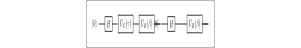
\includegraphics[width=0.6\textwidth]{../../images/qaoa_knapsack_circuit.svg}
\end{center}

\subsection{数学推导}

背包问题的目标函数：
\begin{equation}
\max \sum_i v_i x_i \quad \text{s.t.} \sum_i w_i x_i \leq C
\end{equation}

QAOA 编码：
\begin{equation}
C(x) = \sum_i v_i x_i - \lambda \max(0, \sum_i w_i x_i - C)
\end{equation}

其中 $\lambda$ 是惩罚系数。

\textbf{QAOA 电路}：
\begin{equation}
|\gamma, \beta\rangle = \prod_{l=1}^{p} e^{-i\beta_l B} e^{-i\gamma_l C} |+\rangle^{\otimes n}
\end{equation}

\subsection{几何解释}

QAOA 背包问题在参数空间中寻找最优选择。量子计算机负责制备态和测量，经典优化器负责更新参数。

\section{代码详解}

\begin{verbatim}
from quonic.algorithms import qaoa_knapsack

# qaoa_knapsack(weights, values, capacity, p, optimizer)
# weights: 物品重量
# values: 物品价值
# capacity: 背包容量
# p: QAOA 层数
# optimizer: 优化器

result = qaoa_knapsack(
    weights=[2, 3, 4, 5],
    values=[3, 4, 5, 6],
    capacity=8,
    p=2,
    optimizer='cobyla'
)

# result.max_value: 最大价值
# result.selection: 选择的物品
# result.params: 优化后的参数
print(f'Max value: {result.max_value}')
print(f'Selected items: {result.selection}')
\end{verbatim}

\section{进阶用法}

\subsection{场景 1：不同层数}

\begin{verbatim}
from quonic.algorithms import qaoa_knapsack

weights = [2, 3, 4, 5]
values = [3, 4, 5, 6]
capacity = 8

for p in [1, 2, 4]:
    result = qaoa_knapsack(weights, values, capacity, p=p)
    print(f'p={p}: Max value={result.max_value}')
\end{verbatim}

\subsection{场景 2：不同容量}

\begin{verbatim}
from quonic.algorithms import qaoa_knapsack

weights = [2, 3, 4, 5]
values = [3, 4, 5, 6]

for capacity in [5, 8, 10, 15]:
    result = qaoa_knapsack(weights, values, capacity, p=2)
    print(f'Capacity={capacity}: Max value={result.max_value}')
\end{verbatim}

\subsection{场景 3：大规模问题}

\begin{verbatim}
from quonic.algorithms import qaoa_knapsack
import numpy as np

# 大规模背包问题
n_items = 10
weights = np.random.randint(1, 10, n_items).tolist()
values = np.random.randint(1, 10, n_items).tolist()
capacity = sum(weights) // 2

result = qaoa_knapsack(weights, values, capacity, p=3)
print(f'Max value: {result.max_value}')
\end{verbatim}

\section{适用场景}

\subsection{资源分配}

QAOA 背包问题可以用于资源分配。例如，在有限预算下选择最有价值的项目。

\subsection{投资组合优化}

QAOA 背包问题可以用于投资组合优化。例如，在风险约束下最大化收益。

\section{常见问题}

\subsection{QAOA 背包问题和经典背包问题有什么区别？}

QAOA 背包问题使用量子策略，可以利用量子叠加探索更大的解空间。

\subsection{QAOA 背包问题的精度如何？}

精度取决于层数和参数优化策略。

\section{学习路径}

\subsection{前置知识}
\begin{itemize}
  \item QAOA
  \item 背包问题
  \item 组合优化
\end{itemize}

\subsection{继续学习}
\begin{itemize}
  \item QAOA 旅行商问题
  \item QAOA 最大独立集
  \item 量子优化
\end{itemize}

\section{完整示例代码}

\subsection{示例 1：基本 QAOA 背包问题}

\begin{verbatim}
from quonic.algorithms import qaoa_knapsack

weights = [2, 3, 4, 5]
values = [3, 4, 5, 6]
capacity = 8

result = qaoa_knapsack(weights, values, capacity, p=2)
print(f'Max value: {result.max_value}')
\end{verbatim}

\section{下载}

\begin{itemize}
  \item [qaoa\_knapsack.py](https://github.com/ChrisLee0721/QuoNic/blob/main/examples/qaoa_knapsack/qaoa_knapsack.py)
\end{itemize}

\end{document}
